\chapter{Grundlagen}
Diese Arbeit befasst sich mit Winkeldefekten und ihren Auswirkungen auf die Terminierung des intrinsischen Delaunay-Refinement. Zum Verständnis sind Grundkenntnisse der computergestützten Geometrie und deren Begrifflichkeiten sowie allgemeine mathematische Grundbegriffe erforderlich. Im Folgenden werden daher einige der wichtigsten Grundbegriffe und Definitionen erläutert. Wir orientieren uns dabei in der
Formulierung an den Arbeiten von 
 Bobenko, Springborn, Fisher u. a., Sharp u. a. und Shewchuk
 \cite{Bobenko:2006:SIGGRAPH,Sharp:2019:NIT,Bobenko:2007:LaplaceBeltrami,shewchuk:1997:delaunay,SHEWCHUK:2002:chuws},
wobei wir die Notation im Sinne der Konsistenz dieser Arbeit ggf. anpassen.

\section*{Triangulierung}

Eine Triangulierung $M$, gegeben durch das Tripel $  (V, E, T) $, ist die Zerlegung einer Fläche oder Oberfläche in disjunkte Dreiecksflächen; die Dreiecke sind dabei entlang ihrer Kanten überlappungsfrei verbunden.
Triangulierungen bestehen dabei im Allgemeinem nicht aus uniformen Dreiecken.
Die Vereinigung der disjunkten Dreiecksflächen bildet die zerlegte Fläche. \\  

\begin{figure}[h]%{r}{5cm}
    \centering
  \input{figuren/zulässige_triangulierungen}
  %\setcapindent{0em}
  \caption{Illustration von zulässigen und nicht zulässigen Flächenaufteilungen}
\end{figure}

Dabei bezeichnet  $V$ die Menge der Knoten, $E$ die Menge der Kanten und $T$ die Menge der Dreiecksflächen.


\section*{Auffaltung}
Die Auffaltung eines dreidimensionalen Objektes ist die Ausbreitung der Flächen seiner Oberfläche (oder Teilen davon) in der euklidischen Ebene, nachdem es an einigen Kanten aufgeschnitten worden ist. 

\section*{Gesamtwinkel}
\label{def:gesamtwinkel}
Seien $M = (V, E, T)$ eine Triangulierung, $i,j,k \in V$ und $(i, j),(i, k),(j, k) \in E$, dann bezeichnet $\theta_i^{j,k}$ den Winkel zwischen den Kanten  $(i, j)$ und $(i, k)$ in einem Dreieck. Der Gesamtwinkel $ \Theta_i$ eines Knotens $i$ bezeichnet die Summe aller zu $i$ gehörender Innenwinkel $\theta_i^{j,k}$.

\begin{figure}[H]%{r}{5cm}
    \centering
  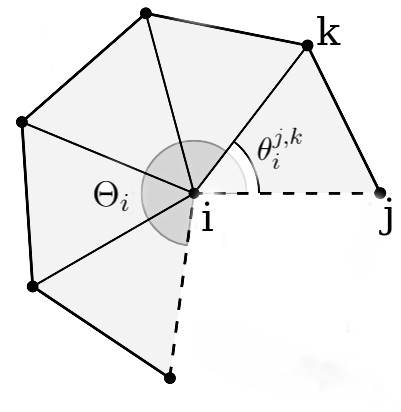
\includegraphics[width=2in]{images/gesammtwinkel.jpg}
  %\setcapindent{0em}
  \caption{Illustration Gesamtwinkel \gesamtwinkel und Innenwinkel  $\theta_i^{j,k}$  eines Knotens $i$  \cite{Sharp:2019:NIT}}
\end{figure}
 
\section*{Winkeldefekt}
\label{def:winkeldefekt}
In der euklidischen Ebene addieren sich die Winkel um einen Knoten zu $2\pi$. Bei einer Oberfläche können die Winkel sich zu weniger oder mehr als $2\pi$ addieren.\\
Dieses Phänomen bezeichnet man in der Geometrie als Winkeldefekt. Für den Gesamtwinkel eines Knotens gilt dann: $\gesamtwinkel* \neq 2\pi$ 

\cite{richeson:2012:euler}.\\
\begin{figure}[H]%{r}{5cm}
    \centering
  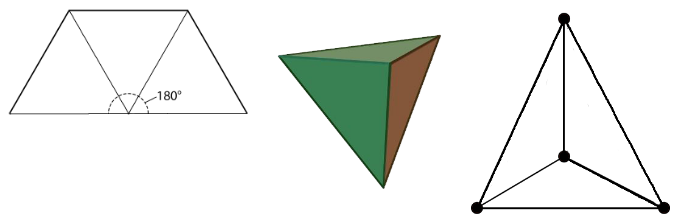
\includegraphics[width=4in]{images/winkeldefekt_polyder_2.png}
  %\setcapindent{0em}
  \caption{Illustration eines Knotens mit Gesamtwinkel $\pi$ und  Winkeldefekt von $\pi$ \cite{Koch_2019_CVPR}}
\end{figure}
 
 Bei einer Oberfläche ist der Winkeldefekt an einem Knoten $i$ gleich $2\pi - \gesamtwinkel* $. 

\begin{definition}(Kegelspitze)\\

Ein Knoten $s \in V$  wird als Kegelspitze bezeichnet, wenn er einen Winkeldefekt hat.\\
 
Es werden zwei Arten von Kegelspitzen unterschieden:
 \begin{itemize}
     \item sphärische Kegelspitzen, falls $\Theta_s < 2\pi $ und 
     \item hyperbolische Kegelspitzen, falls $\Theta_s > 2\pi $ .
 \end{itemize} 


\begin{figure}[h]%{r}{5cm}
    \centering
  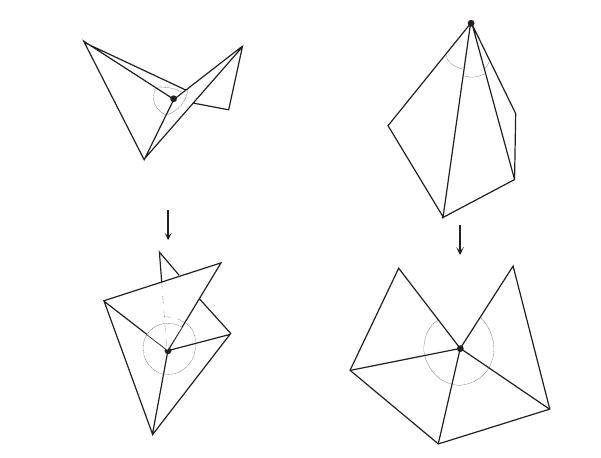
\includegraphics[width=3in]{images/Merged_document.png}
  %\setcapindent{0em}
  \caption{Links hyperbolische Kegelspitze und rechts sphärische Kegelspitze   \cite{Polthier:2006:SIGGRAPH}}
\end{figure}
 

\end{definition}

\section*{Delaunay-Triangulierung einer stückchenweise flachen Oberfläche}
\begin{figure}[H]%{r}{5cm}
    \label{fig:hase}
    \centering
    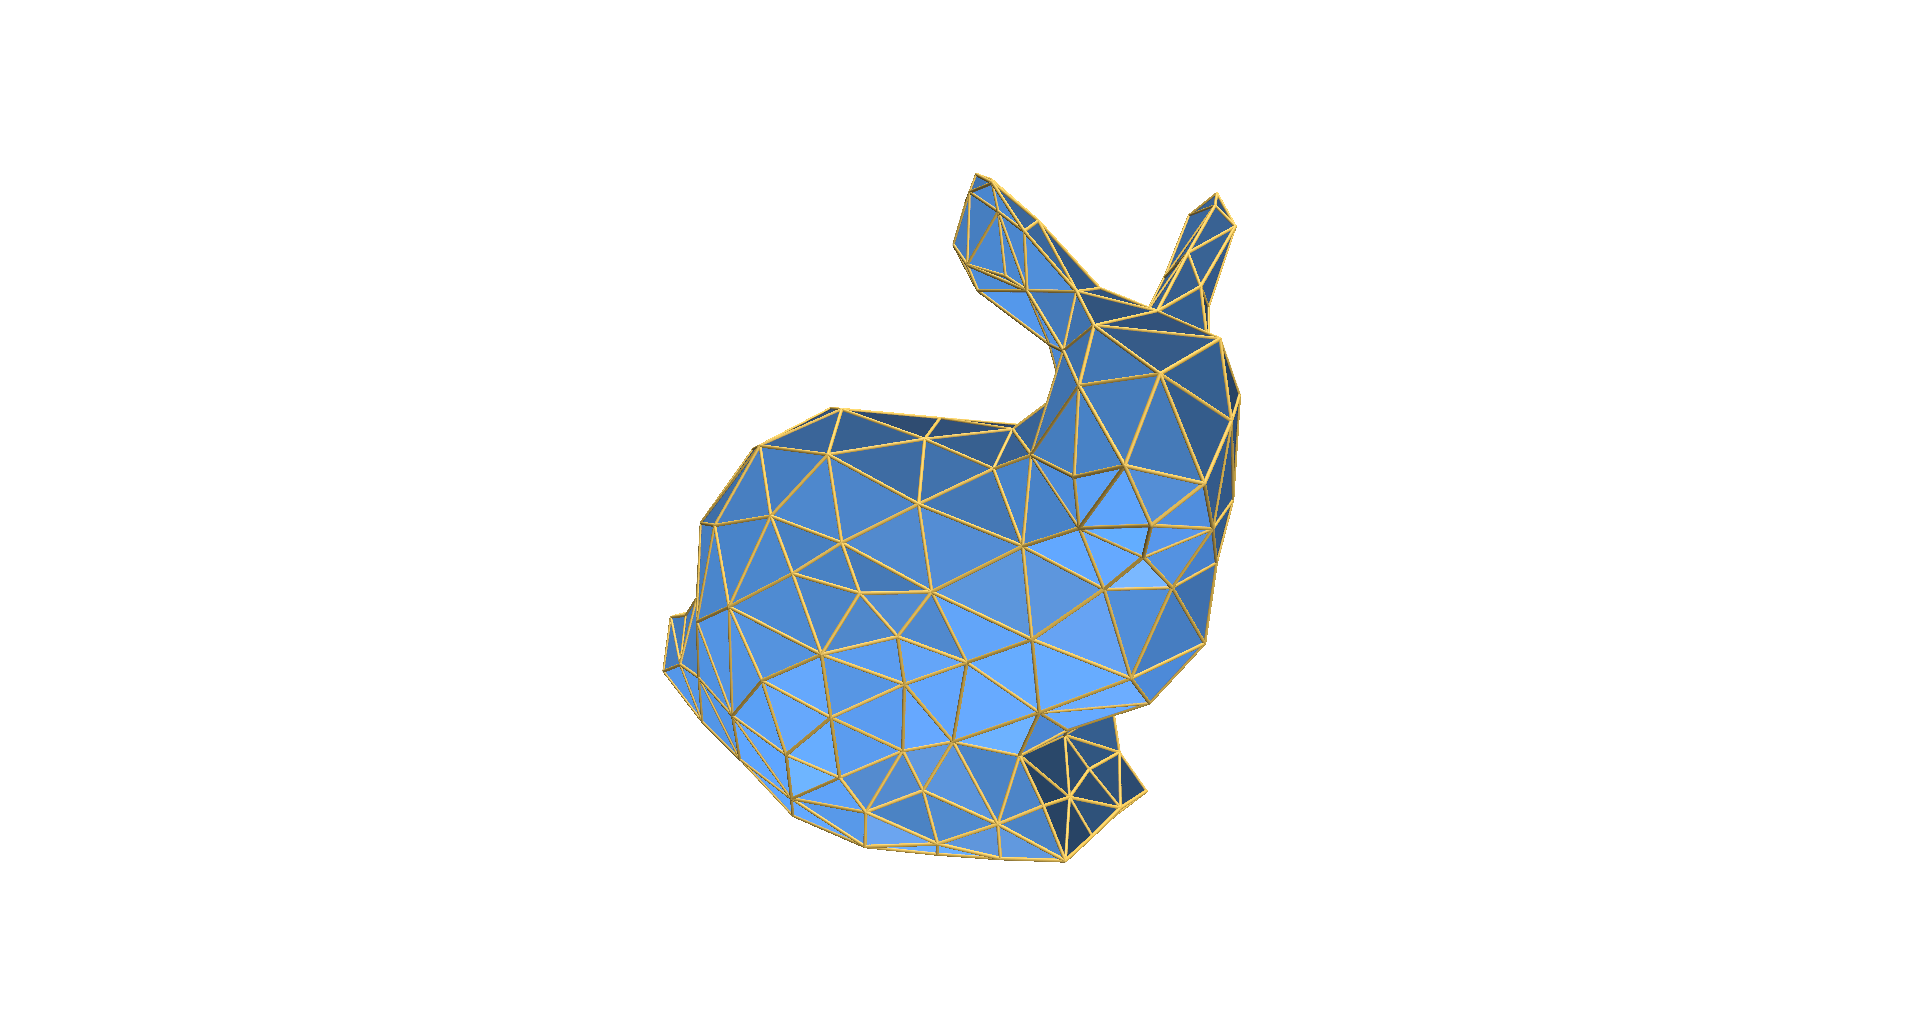
\includegraphics[width=5in]{images/image1.png}
  %\setcapindent{0em}
  \caption{Illustration der Triangulierung einer stückchenweise flachen Oberfläche}
\end{figure}

\subsection*{Stückchenweise flache Oberflächen (StF-Oberflächen)}

Stückweise flache Oberflächen wie in Abbildung \ref{fig:hase} gezeigt sind 2-Mannigfaltigkeit mit kegelspitzenartigen Singularitäten. Intuitiv bedeutet das, dass diese Flächen lokal euklidisch sind außer an einigen singulären Punkten. Dort verhalten sie sich wie eine sphärische oder hyperbolische Kegelspitze. Kegelspitzen können im Allgemeinen dort auftreten, wo Linien zusammengeführt werden (siehe Abbildung \ref{fig:hase}).

\subsection*{Triangulierung  einer  StF-Oberfläche}
Sei $M = (V,E,T)$ eine Triangulierung einer StF-Oberfläche. Dann gilt für die Menge der Kegelspitzen $S$ der StF-Oberfläche, dass $S \subset V$.\\ 
 
Die Triangulierung einer Stf-Oberfläche ist für gewöhnlich eine Sammlung von ebenen Dreiecken im Raum (siehe Abbildung \ref{fig:hase}). Dies ist jedoch keine Anforderung an die Triangulierung, es wird lediglich gefordert, dass die Möglichkeit existiert, jede Fläche als Dreieck in der euklidischen Ebene aufzufalten. \\  

Auf $M$ sind also auch sogenannte irreguläre Dreiecke erlaubt, bei denen (zum Beispiel) ein Knoten eine (irreguläre) Kante zu sich selbst hat und die anderen beiden Kanten gleich sind oder alle drei Knoten identisch sind (siehe Abb. \ref{fig:auffaltung_irregulaer}).
Formal ist $M$  somit ein $\Delta$-Komplex \cite[abschnitt 2.1]{hatcher:2005:deltakomplex}.\\
 
\begin{figure}[H]%{r}{5cm}
    \centering
  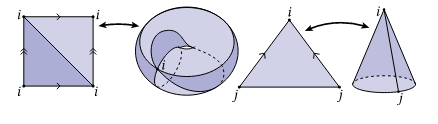
\includegraphics[width=4in]{images/auffaltung_irregulaer.png}
  %\setcapindent{0em}
  \caption{Illustration von irregulären Dreiecken, die sich in der  euklidischen Ebene zu gewöhnliche Dreiecken auffalten \cite{Sharp:2019:NIT}}
\label{fig:auffaltung_irregulaer}
\end{figure}
% in der Geometrie bezieht sich intrinsische darauf, dass (zum Beispiel) Oberflächen ohne Bezug auf ihre Lage im Raum beschrieben werden, wobei nur Messungen entlang der Oberfläche (Längen, Winkel usw.) verwendet werden.\\


\begin{definition}(Eingebettete leere Kreisscheibe)\\
Sei $M = (V,E,T)$ eine Triangulierung einer StF-Oberfläche.
Eine eingebettete leere Kreisscheibe ist eine stetige Abbildung $\phi: k^{\ast} \rightarrow M$, wobei $k$ eine offene runde Scheibe in der euklidischen Ebene und  $k^{\ast}$ ihr Abschluss ist.
Jeder $v \in K$ hat eine Nachbarschaft, die isometrisch abgebildet wird. Es gilt $\phi (k) \cap V = \emptyset $. Folglich sind alle Punkte in $\phi^-1(V)$ im Rand von $K$ enthalten: $\phi^{-1}(V) \subset \partial K $ 
\end{definition} 
 
 
 

\subsection*{Delaunay-Triangulierung einer geschlossenen StF-Oberfläche}
Sei $M = (V,E,T)$ eine Delaunay-Triangulierung einer geschlossenen StF-Oberfläche.
Die Delaunay-Triangulierung ist dabei eine Zerlegung der StF-Oberfläche in disjunkte Teilmengen und besteht aus folgenden Mengen: Eine Teilmenge $ C \subset M$ ist eine geschlossene Zelle der Delaunay-Triangulierung genau dann, wenn eine eingebettete leere Kreisscheibe $\phi: k^{\ast} \rightarrow M$ existiert, sodass $\phi^{-1}(M) \not = \emptyset$ und auf ihrem Rand genau die Elemente aus $C$ liegen. 
$C$ ist also das Bild der konvexen Hülle von $\phi^{-1}(M)$.
Dabei unterscheidet man die Zellen an der Anzahl ihrer Knoten: 1-Zellen (Knoten), 2-Zellen (Kanten) und 3-Zellen (Flächen).\\   

Aufgrund ihrer nützlichen Eigenschaften ist die  Delaunay-Triangulierung  eine der in der Praxis am häufigsten eingesetzten Triangulierungen. 
Die Eigenschaften sind unter anderem:

\begin{itemize}
    \item die Dualität zum Voronoidiagramm (siehe Abb. \ref{fig:delaunay_voronoi}  ) \cite{indermitte:2001:voronoi,aurenhammer:2000:voronoi}
    \item die Eigenschaft der leeren Kreisscheibe (im folgenden Delaunay-Eigenschaft genannt)\\(siehe Abb. \ref{fig:delaunay_umkreis})
    \item sie ist in der Regel eindeutig (siehe Abb. \ref{fig:eindeutig})
    \item jede beliebige Triangulierung kann mit einer endlichen Zahl an Kantenflips in eine Delaunay-Triangulierung überführt werden. Dies gilt für die euklidische Ebene \cite{shewchuk:1997:delaunay} und für die StF-Oberfläche \cite{Bobenko:2007:LaplaceBeltrami}.
    \item eine Kante ist genau dann Teil der Delaunay-Triangulierung,  wenn sie die Delaunay-Eigenschaft erfüllt. 
    \item unter allen möglichen Triangulierungen ist die Delaunay-Triangulierung diejenige, welche den minimalen Innenwinkel über alle Dreiecke maximiert. 
    %\item die Maximierung des minimalen Innenwinkels über alle Dreiecke. Letztere Eigenschaft verhindert in weiterer Folge Rundungsfehler.
\end{itemize}
 
 
 \begin{figure}[H]
    \centering
    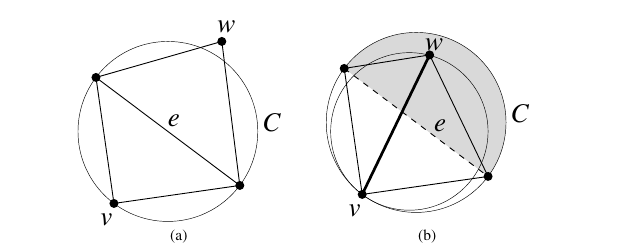
\includegraphics[width=5in]{images/lokal_delaunay.png}
    \caption{Illustration: dass jede Kante, Kante die geflippt werden muss geflipt werden kann. in $(a)$ erfüllt $e$ die Delaunay-Eigenschaft. in $(b)$ erfüllt $e$ sie nicht kann, aber die durch den Kantenflip erzeugt Kante erfüllt die Delaunay-eigenschaft \cite{shewchuk:1997:delaunay} }
    \label{fig:lokal_delaunay}
\end{figure}


\begin{figure}[h]%{r}{5cm}
    \centering
  \includesvg[width=2in]{images/Delaunay_Voronoi}
  %\setcapindent{0em}
  \caption{ Umkreismittelpunkte der Dreiecke der Delaunay-Triangulierung sind die Knoten  der Voronoizellen.\cite{Hferee:2011:delaunay-voronoi}}
  \label{fig:delaunay_voronoi}
\end{figure}

\begin{figure}[H]%{r}{5cm}
    \centering
  \includesvg[width=2.5in]{images/Delaunay_circumcircles}
  %\setcapindent{0em}
  \caption{Der Umkreis eines Dreiecks ist die einzige Kreisscheibe, die durch die drei Eckknoten des Dreiecks verläuft. Die Delaunay-Triangulierung ist die Triangulierung, bei der jedes Dreieck einen leeren Umkreis (Kreisscheibe) besitzt. D. h. die Fläche der Kreisscheibe enthält keine anderen Knoten der Triangulierung. \cite{Gjacquenot:2013:delaunay-circumcircles}}
  \label{fig:delaunay_umkreis}
\end{figure}
    
    
\begin{figure}[H]
    \centering
    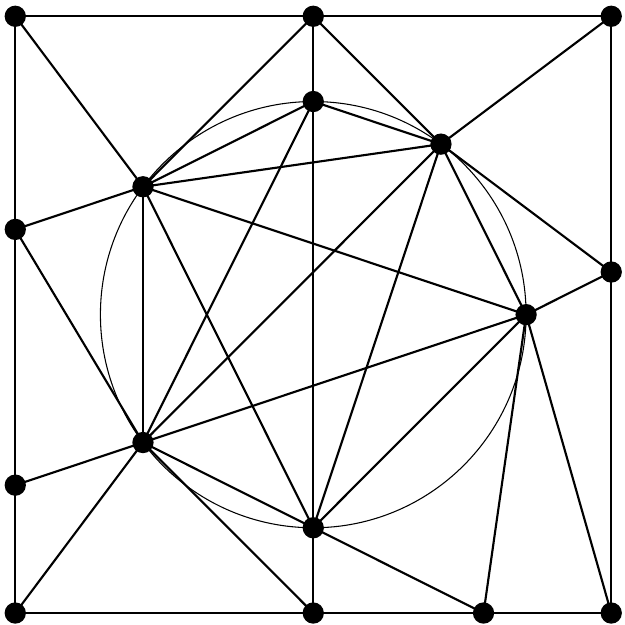
\includegraphics[width=2in]{images/Bildschirmfoto von 2021-11-27 22-34-40.png}
    \caption{ Wenn mehr als drei Punkte auf dem Rand derselben Kreisscheibe liegen, ist die Delaunay Triangulierung nicht eindeutig. Da dies in der  Praxis selten vorkommt, treffen wir die vereinfachte Annahm, dass niemals mehr als drei Punkte auf einer Kreisscheibe liegen\cite{shewchuk:1997:delaunay} }
    \label{fig:eindeutig}
\end{figure}
    
\newpage

Die Qualität der Triangulierung definiert sich über das Verhältnis der  Innenwinkel- und Flächenverteilung der einzelnen Dreiecke. 
Da die durch die Delaunay-Triangulierung maximierten Innenwinkel über alle Dreiecke einer festen Knotenmenge noch zu klein sein könnten, 
kann die Qualität darüber hinaus verbessert werden. Dies kann über das gezielte Einfügen weiterer Knoten geschehen. Hierfür werden Delaunay-Refinement Algorithmen verwendet.\\

 





